% !TeX TS-program = xelatex

\documentclass{beamer}
\usetheme{metropolis}

\usepackage{multicol}

\usepackage{ragged2e} % who justifies the text
\usepackage{xecolor}
\usepackage{amsmath}
%\usefonttheme[onlymath]{serif} %Change the math font

\usepackage{tabularx}
\usepackage{booktabs}
\usepackage[style=numeric,sorting=ynt]{biblatex}
\addbibresource{references.bib}
\usepackage{xepersian}
\settextfont{Vazir}
\setlatintextfont{Roboto}

%---------------------------------------------------------------------------------
% Colors
%---------------------------------------------------------------------------------
\definecolor{orange}{RGB}{255, 165, 0}
\definecolor{green}{RGB}{124, 252, 0}
\definecolor{cyna}{RGB}{0, 255, 255}

%---------------------------------------------------------------------------------
% Seetings to force Beamer works with Xepersian and RTL typesetting
%---------------------------------------------------------------------------------
%\raggedleft

% For right to left lists (itemize and enumerate)
\makeatletter
\newcommand{\RTList}{\raggedleft\rightskip\@totalleftmargin}
\makeatother
% Correct the bullet for RTL texts
\setbeamertemplate{itemize item}{\scriptsize\raise1.25pt%
 \hbox{\donotcoloroutermaths$\blacktriangleleft$}} 

% To force beamer use numbering in captions
\setbeamertemplate{caption}[numbered]{}% Number float-like environments

\setbeamertemplate{footline}[frame number]
\setbeamertemplate{section in toc}[circle]
\setbeamertemplate{blocks}[rounded][shadow=true]
\setbeamercolor{block body}{bg=lightgray}
\setbeamercolor{headline}{bg=orange}
\setbeamersize{text margin left=1cm,text margin right=1cm}

\setbeamertemplate{headline}
{
    \begin{beamercolorbox}{section in head/foot}
        \vspace{2pt}\insertnavigation{\paperwidth}\vspace{2pt}
    \end{beamercolorbox}
}
  
%---------------------------------------------------------------------------------
% To force beamer use numbering in captions
\setbeamertemplate{caption}[numbered]{}% Number float-like environments

\setbeamertemplate{footline}
{%
  \leavevmode%
  \hbox{%
    \begin{beamercolorbox}[wd=.333333\paperwidth,ht=2.25ex,dp=1ex,center]{author in head/foot}%
      \usebeamerfont{author in head/foot}\insertshortauthor%
    \end{beamercolorbox}%
    \begin{beamercolorbox}[wd=.333333\paperwidth,ht=2.25ex,dp=1ex,center]{title in head/foot}%
      \usebeamerfont{title in head/foot}\insertshorttitle%
    \end{beamercolorbox}%
    \begin{beamercolorbox}[wd=.333333\paperwidth,ht=2.25ex,dp=1ex,right]{date in head/foot}%
      \usebeamerfont{date in head/foot}\insertsection\hspace*{2em}
      \insertframenumber{} / \inserttotalframenumber\hspace*{2ex}
    \end{beamercolorbox}
  }%
}
\setbeamertemplate{section in toc}[circle]
\setbeamertemplate{blocks}[rounded][shadow=true]
\setbeamercolor{block title}{bg=orange}
\setbeamercolor{block body}{bg=lightgray}
\setbeamersize{text margin left=1cm,text margin right=1cm}

%---------------------------------------------------------------------------------
\title{نیازمندی کیفیت سرویس در کارکردهای مجازی شبکه}
\subtitle{}
\author{پرهام الوانی}
\institute{%
    دانشکده مهندسی کامپیوتر\\
    دکتر بهادر بخشی
}
\date{\today}
\titlegraphic{\vspace{4.5cm}\flushleft
\includegraphics[height=50pt]{images/logo}}

\begin{document}

\makeatletter

\setbeamertemplate{title}{%
	\linespread{1.0}%
	\inserttitle%
	\par%
	\vspace*{0.5em}
}
\setbeamertemplate{subtitle}{%
	\insertsubtitle%
	\par%
	\vspace*{0.5em}
}

\AtBeginSection[]
{%
	\begin{frame}{فهرست}
		\tableofcontents[currentsection]
	\end{frame}
	\begin{frame}
		\begin{center}
			\insertsectionnumber. \insertsection%
		\end{center}
		\usebeamertemplate*{title separator}
	\end{frame}
}

\makeatother


\begin{persian}
	%------------------------------------------
	% Title frame (0)
	%------------------------------------------
	{%
		\setbeamertemplate{footline}{}
		\begin{frame}
			\titlepage%
		\end{frame}
	}

	%-------------------------------------------------------------------------------
	\begin{frame}{فهرست}
		\tableofcontents[pausesections]
	\end{frame}

	%-------------------------------------------------------------------------------
	\section{مقدمه}

	%-------------------------------------------------------------------------------
	\begin{frame}{شبکه‌های سنتی}
		\begin{itemize}\RTList{}
			\justifying
			\item
			      یک سرویس شبکه به صورت تعدادی
			      \textcolor{orange}{کارکرد مشخص}
			      که ترافیک با
			      \textcolor{orange}{ترتیب مشخصی}
			      از آن ها عبور می‌کند، تعریف می‌شود.
			\item
			      کارکردهای شبکه به صورت سخت‌افزار و نرم‌افزار اختصاصی تهیه شده
			      از سازندگان مختلف استفاده می‌شوند.
			\item
			      کارکردها باید در \textcolor{green}{مکان} مناسب در شبکه قرار گیرند و ترافیک به سمت
			      آن‌ها \textcolor{green}{هدایت} شود.
		\end{itemize}
	\end{frame}

	%-------------------------------------------------------------------------------
	\begin{frame}{شبکه های سنتی}
		\begin{itemize}\RTList{}
			\justifying
			\item
			      افزایش نیازمندی به سرویس‌های
			      \textcolor{orange}{متنوع}
			      با
			      \textcolor{green}{عمرکوتاه}
			      و
			      \textcolor{cyna}{نرخ بالای ترافیک}
			      \begin{itemize}\RTList{}
				      \item خریداری، انبارداری و استقرار سخت‌افزارهای اختصاصی
				      \item افزایش هزینه‌های خرید، آموزش و انبارداری
				      \item کاهش فضای فیزیکی
				      \item سربار آموزش کارکنان
				      \item محدودیت نوآوری در سخت‌افزار و سرویس
			      \end{itemize}
		\end{itemize}
		\begin{block}{}
			\centering
			\lr{Network Functions Virtualization}\\
			مجازی‌سازی کارکردهای شبکه
		\end{block}
	\end{frame}

	%-------------------------------------------------------------------------------
	\begin{frame}{شبکه های سنتی}
		\begin{itemize}\RTList{}
			\justifying
			\item ترافیک کاربر باید از تعدادی کارکرد شبکه به ترتیب معینی عبور کند.
			\item کارکردها به صورت سخت‌افزاری به یکدیگر متصل هستند و ترافیک با استفاده از جداول مسیریابی به سمت آن‌ها هدایت می‌شود.
			\item نیاز به تغییر همبندی سریع و یا مکان کارکردها برای سرویس‌دهی بهتر
			      \begin{itemize}\RTList{}
				      \item استقرار و تغییر ترتیب کارکردها دشوار است
				      \item امکان رخدادن خطاهای متعدد
			      \end{itemize}
		\end{itemize}
		\begin{block}{}
			\centering
			\lr{Service Function Chaining}\\
			زنجیره‌سازی کارکرد سرویس
		\end{block}
	\end{frame}

	%-------------------------------------------------------------------------------
	\begin{frame}{معماری پیشنهادی}
		\begin{itemize}\RTList{}
			\justifying
			\item مجازی‌سازی کارکردهای شبکه
			      \begin{itemize}\RTList{}
				      \item اواخر سال ۲۰۱۲، \lr{ETSI NFV ISG} توسط هفت اپراتور جهانی شبکه تأسیس شد.
				      \item اکنون بیش از 250 سازمان با آن همکاری می‌کنند.
				      \item اجرای کارکردها بر روی سرورهای استاندارد با توان بالا به وسیله مجازی‌سازی کارکردها
				            \begin{itemize}\RTList{}
					            \item کاهش نیاز به تجهیزات سخت‌افزاری خاص منظوره
					            \item اشتراک گذاری منابع بین کارکرد‌ها
					            \item کاهش هزینه‌های تجهیزات و مصرف انرژی از طریق تجمیع کارکردها
				            \end{itemize}
			      \end{itemize}
		\end{itemize}
	\end{frame}

	%-------------------------------------------------------------------------------
	\begin{frame}{معماری پیشنهادی}
		\begin{itemize}\RTList{}
			\justifying
			\item زنجیره‌سازی کارکرد سرویس
			      \begin{itemize}\RTList{}
				      \item امکان تعریف زنجیره کارکردها به صورت پویا و بدون تغییر در زیرساخت فیزیکی
				      \item قابل اجرا بر بستر \textcolor{green}{شبکه‌های سنتی} یا \textcolor{orange}{نرم‌افزار بنیان}
				      \item \lr{RFC 7665}
			      \end{itemize}
		\end{itemize}
	\end{frame}

	%-------------------------------------------------------------------------------
	\begin{frame}{معماری پیشنهادی}
		\begin{itemize}\RTList{}
			\justifying
			\item \cite{Yang2021}
			\item زنجیره‌های مرتب تمام
			\item زنجیره‌های مرتب جزئی
		\end{itemize}
		\begin{center}\begin{figure}
				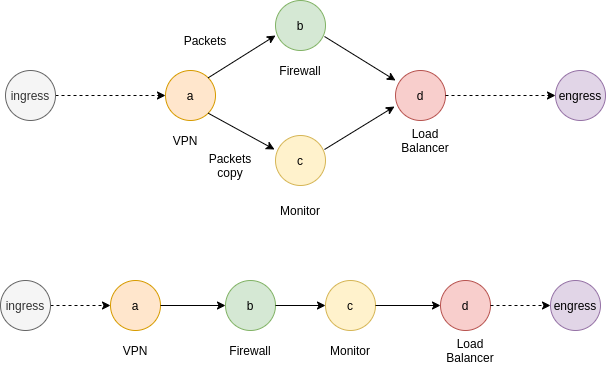
\includegraphics[scale=0.3]{images/partially-totally-sfc.png}
				\caption{زنجیره‌های مرتب جزئی و کامل}
			\end{figure}\end{center}
	\end{frame}

	%-------------------------------------------------------------------------------
	\begin{frame}{معماری پیشنهادی}
		\begin{center}\begin{figure}
				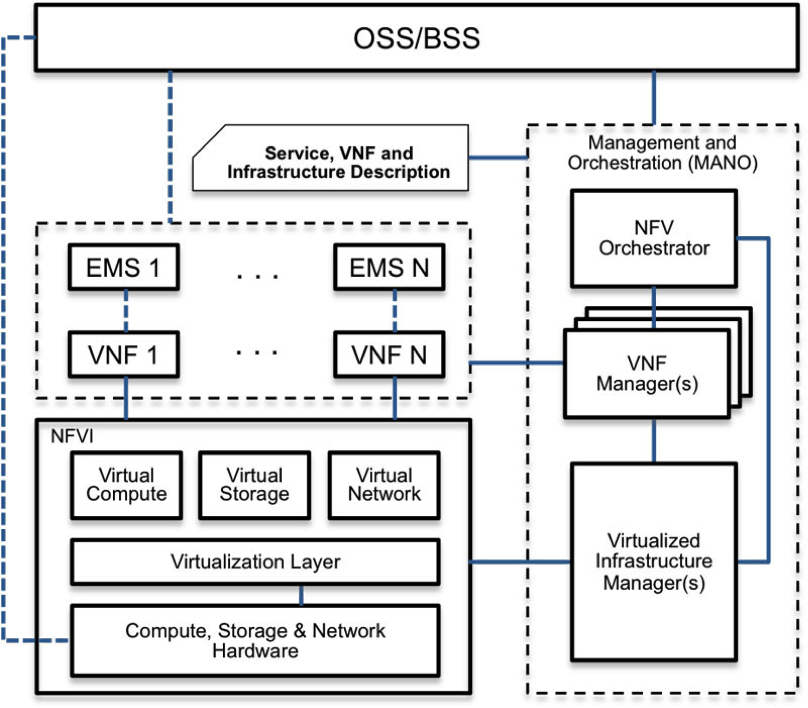
\includegraphics[scale=0.5]{images/nfv-arch.png}
				\caption{معماری سطح بالای مجازی‌سازی کارکردهای شبکه}
			\end{figure}\end{center}
	\end{frame}

	%-------------------------------------------------------------------------------
	\begin{frame}{معماری پیشنهادی}
		\begin{itemize}\RTList{}
			\justifying
			\item \lr{NFVO} وظیفه‌ی استقرار زنجیره‌های کارکرد سرویس را برعهده دارد.
			\item \lr{VNFM} مسئول چرخه‌ی زندگی کارکردهای مجازی شبکه می‌باشد.
		\end{itemize}
	\end{frame}

	%-------------------------------------------------------------------------------
	\begin{frame}{تخصیص منابع}
		\begin{itemize}\RTList{}
			\justifying
			\item
			      جایگذاری کارکردهای مجازی شبکه به همراه مسیریابی ترافیک\\
			      \begin{center}\footnotesize\lr{VPTR: VNF Placement and Traffic Routing}\end{center}
			\item
			      جایگذاری کارکردهای مجازی شبکه\\
			      \begin{center}\footnotesize\lr{VNFP: VNF Placement}\end{center}
			\item
			      مسیریابی ترافیک\\
			      \begin{center}\footnotesize\lr{TRR: Traffic Routing}\end{center}
			\item
			      بازاستقرار و تثبیت کارکردهای مجازی شبکه\\
			      \begin{center}\footnotesize\lr{VRC: VNF Redeployment and Consolidation}\end{center}
		\end{itemize}
	\end{frame}

	%-------------------------------------------------------------------------------
	\begin{frame}{اهداف}
		\begin{itemize}\RTList{}
			\justifying
			\item هزینه
			      \begin{itemize}\RTList{}
				      \item مساله‌ی پایه‌ای در بحث تخصیص منابع
				      \item وجود جواب با برآورده شدن محدودیت‌های نودها و لینک‌ها
				      \item \lr{NP-Hard}
			      \end{itemize}
			\item \textcolor{green}{کیفیت سرویس}
			      \begin{itemize}\RTList{}
				      \item \textcolor{orange}{تاخیر}
						\begin{itemize}\RTList{}
							\item انتشار
							\item انتقال
							\item صف
							\item پردازش
						\end{itemize}
				      \item دسترسی پذیری
			      \end{itemize}
		\end{itemize}
	\end{frame}

	%-------------------------------------------------------------------------------
	\section{مراجع}

	%-------------------------------------------------------------------------------
	\begin{frame}{}
		\begin{latin}
		\printbibliography%
		\end{latin}
	\end{frame}

\end{persian}
\end{document}